\chapter{Discussion}
\label{chap:discussion}

In this chapter, we will conclude the user study with a discussion of its results and suggest possible future improvements both to the study and to mesh difference visualizations in general.

%%-----------------------------------------------------------------------------------------
%% SECTION
%%-----------------------------------------------------------------------------------------
\section{Significant Results}
\label{sec:discussion-sig_results}

The study has yielded three significant results which show the contribution of~visualizations in general and also a good performance of the newly presented visualizations of vector-based difference metrics.

%%-----------------------------------------------------------------------------------------
\subsection{The Overall Contribution of Visualizations}
\label{subsec:discussion-sig_results-overall_contrib}

The answers to question 7 (see attachment \ref{attch:complete_study_results-question7}), which requires participants to click on the face which has larger cheekbones, has shown an overwhelming dominance of visualizations over raw triangle meshes. Any of the three types of~visualizations presented helped participants to answer correctly, whereas when no visualization was shown, answers were almost equally distributed among all the possible options. Moreover, when participants were shown meshes without a~visualization, it took them longer to arrive at an answer. Similar effect could be observed in the answers to question 8 (see attachment \ref{attch:complete_study_results-question8}).

%%-----------------------------------------------------------------------------------------
\subsection{The Contribution of Arrows}
\label{subsec:discussion-sig_results-arrow_contrib}

Question 9 (see attachment\ref{attch:complete_study_results-question9}) has shown a contribution of arrows which we did not include in our expectations (see section \ref{sec:analysis-visualizations}). The question was aimed at the absolute value of the difference and where this value was the smallest. Thresholding performed well as expected but most correct answers were given when arrows were displayed. This shows that the length of an arrow is much more suggestive than the color scale when capturing the absolute value of a difference metric.

See Fig. \ref{fig:meshdiff-normal_projected} for a comparison between color-based and arrow-based visualization of the absolute value of a difference metric.

\begin{figure}[h]
	\centering
	\begin{subfigure}{0.4\textwidth}
		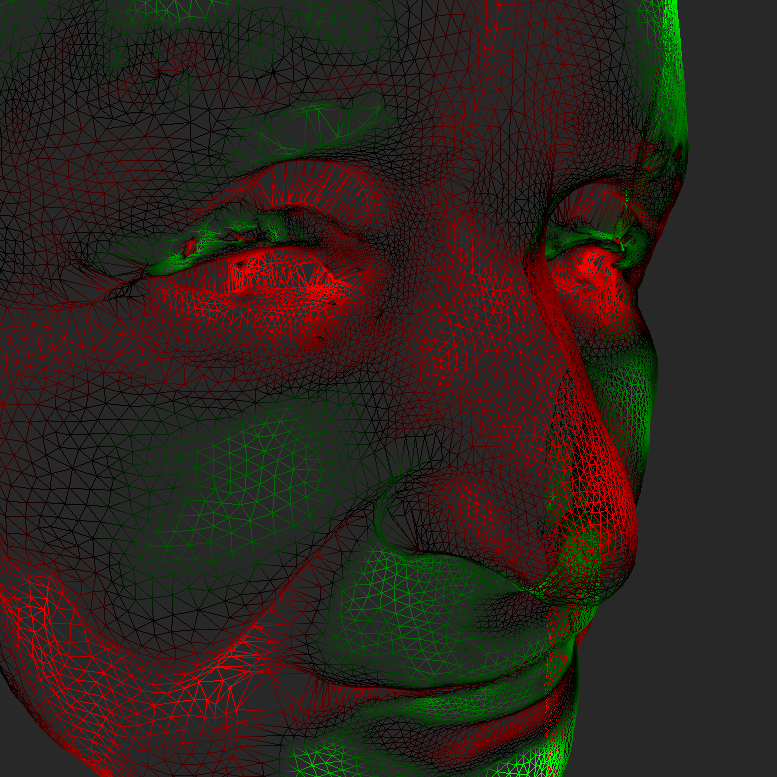
\includegraphics[width=\textwidth]{./img/normal_projected_vis-color.PNG}
		\caption{Color-based}
	\end{subfigure}
	\qquad
	\begin{subfigure}{0.4\textwidth}
		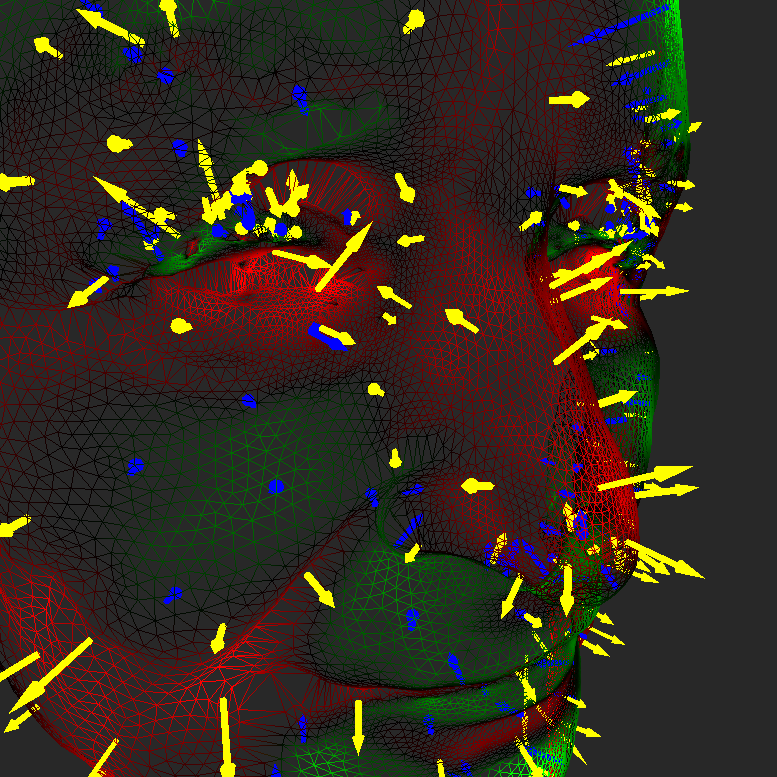
\includegraphics[width=\textwidth]{./img/normal_projected_vis-arrows.PNG}
		\caption{Arrow-based, combined}
	\end{subfigure}
	\caption[MeshDiff - Absolute metric value visualizations]{MeshDiff - Visualizations of corresponding vertex distance projected into surface normal}
	\label{fig:meshdiff-normal_projected}
\end{figure}

%%-----------------------------------------------------------------------------------------
\subsection{The Contribution of Thresholding}
\label{subsec:discussion-sig_results-thresholding_contrib}

In question 3 (see attachment \ref{attch:complete_study_results-question3}), we tried to assess the performance of thresholding in the visualization of the largest difference, a task which it was expected to excel at (see section \ref{sec:analysis-visualizations}). We found that when the threshold was set just under the largest metric value and clusters whose area was too small were excluded too\footnotemark, it was very easy for participants to identify the correct location. On the other hand, when a basic color visualization without thresholding was shown, the spread of answers was significantly larger and participants took much longer to answer. Besides this result, there are two interesting points associated with this question which we have to mention here:

\footnotetext{In our data set, areas by the edge of a mesh are not very representative of the original object they represent because of the way they are cut. At the same time, however, they are very dense and have very high and variable metric values. This results in small clusters which can be easily excluded by area thresholding.}

\begin{itemize}
	\item The answers given for visualization \ref{fig:study-2-5} clearly show that participants were unsure what is meant by ``left'' and ``right'', even though this was explained at the beginning of the study. Because of this, we considered both ``left cheek'' and ``right cheek'' to be correct answers for this particular visualization.
	\item Answers provided when no visualization was shown suggest that this question is beyond the power of basic difference metrics we worked with in this thesis. The reason for this is that the term ``difference'' can be interpreted more globally. Humans in general are very sensitive to facial features and tend to see the difference between them globally, unlike our difference metrics which are local. This could also be observed in the answers to question 9 (see attachment \ref{attch:complete_study_results-question9}).
\end{itemize}

We will further address these and other problematic points in the following sections.

%%-----------------------------------------------------------------------------------------
%% SECTION
%%-----------------------------------------------------------------------------------------
\section{Study Improvements}
\label{sec:discussion-study_improvements}

Because of time constraints, we were not able to improve the study and conduct it again in order to obtain a more complete and thorough comparison between color-based and arrow-based visualizations. A more detailed study would also be able to capture the differences between various clustering methods and clustering parameters which was beyond the resolving power of our study. In this section, we propose several improvements which might help to create such a study.

The most obvious limitation of our study was its scale. However, several other circumstances have further hindered our findings:

\begin{itemize}
	\item The overall presentation of the study did not attract enough attention. For~the next study, we recommend to design a web application with a~modern and responsive interface which would allow for the sessions to be shorter, easier and more accessible to the participants. Being presented with a~modern web application also adds to the feeling that the subject of the study is modern and relevant.
	\item A special attention should be given to the introduction of the study. Our~results, such as \ref{attch:complete_study_results-question3}, have shown that even though the way directions are given was explained in the introductory text, the participants had problems with this. This introduced error into the provided answers. We recommend to create an interactive introduction, rather than text-based, to increase its effectiveness.
	\item The last point related to user experience, which we believe is key, is the way questions are worded. Questions 4 (\ref{attch:complete_study_results-question4}) and 5 (\ref{attch:complete_study_results-question5}) have proven to be too complicated because of the amount of directions and concepts included in them. An example of a good question is question 7 (\ref{attch:complete_study_results-question7}).
	\item Apart from user experience issues which introduced error, we have also noticed a problem with the focus of the study. Our study has mixed questions related to visualizations (e.g. question 6 \ref{attch:complete_study_results-question6}) with questions related to metrics (e.g. question 3 \ref{attch:complete_study_results-question3}). On one hand, this has allowed us to capture the need for more sophisticated difference metrics, on the other hand, it has not contributed to the comparison between various visualization types which is the core of the this thesis.
	\item Another problem related to this is the choice of data. As was mentioned in section \ref{subsec:discussion-sig_results-thresholding_contrib}, the difference metrics we have studied are not suitable for capturing the difference between human faces which people usually tend to see. While these metrics might still be useful in certain cases, this is not very clear from our study because of the data set chosen. We recommend to use more neutral objects in order to eliminate this phenomenon.
\end{itemize}

%%-----------------------------------------------------------------------------------------
%% SECTION
%%-----------------------------------------------------------------------------------------
\section{Method Improvements}
\label{sec:discussion-method_improvements}

In order to improve the new visualizations presented in this thesis, a more detailed user study, as outlined above, should be conducted. However, during the course of~our work we have discovered other possible improvements which are out of~the scope of this thesis. We present these here.

\begin{itemize}
	\item The clustering process used in our visualizations (see section \ref{subsec:analysis-field_clustering-our_method}), more specifically the dendrogram, allows for an interactive visualization to be created. The user would be presented with the visualization of only one cluster covering the whole mesh. By clicking on a cluster, its children in the dendrogram would replace the cluster in the visualization. This would result in a clustering of adaptive detail depending on the specific needs of~the user.
	\item As mentioned in section \ref{subsec:discussion-sig_results-thresholding_contrib}, difference metrics included in this thesis are not sufficient in certain cases, such as when measuring the difference between facial features. A possible next step would be to devise global difference metrics which would better correspond to the idea of shape differences that humans have. As a consequence, clustering would not be required because information would be inherently reduced.
\end{itemize}
